\problemname{J: Frosting on the Cake}
\balloon{ac8dce}

\noindent
Iskander the Baker is decorating a huge cake, covering the rectangular
surface of the cake with frosting.  For this purpose, he mixes frosting
sugar with lemon juice and food coloring, in order to produce three kinds of
frosting: yellow, pink, and white. These colors are identified by the
numbers 0 for yellow, 1~for pink, and 2 for white.

To obtain a nice pattern, he partitions the cake surface into
vertical stripes of width $A_1, A_2, \dots, A_n$ centimeters, and
horizontal stripes of height $B_1, B_2, \dots, B_n$ centimeters, for
some positive integer~$n$. These stripes split the cake surface
into $n\times n$ rectangles. The intersection of vertical stripe~$i$ and
horizontal stripe~$j$ has color number $(i+j) \bmod 3$ for all $1 \leq
i,j \leq n$. To prepare
the frosting, Iskander wants to know the total surface in square
centimeters to be colored for each of the three colors, and asks for your
help.

\begin{center}
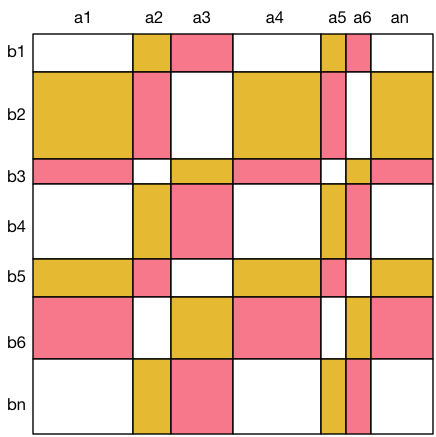
\includegraphics[width=8cm]{Frosting.pdf}
\end{center}

\subsection*{Input}

The input consists of the following integers:
\begin{itemize}
\item on the first line: the integer $n$,
\item on the second line: the values of $A_1,\dots,A_n$, $n$ integers
  separated with single spaces,
\item on the third line: the values of $B_1,\dots,B_n$, $n$ integers separated with 
  single spaces.
\end{itemize}

\subsection*{Limits}

The input satisfies $3\leq n \leq 100\,000$ and
$1 \leq A_1,\ldots,A_n,B_1,\ldots,B_n \leq 10\,000$.

\subsection*{Output}

The output should consist of three integers separated
with single spaces,
representing the total area for each color 0, 1, and 2.

\clearpage
